% Math 402/502 Homework



\documentclass[11pt]{amsart}


\pagestyle{empty}
\thispagestyle{empty}

\usepackage{graphicx}

\usepackage{amsmath}
\usepackage{amssymb}
\usepackage{latexsym}
\usepackage{amsopn}
\usepackage{amsthm}
\usepackage{tikz}
\usetikzlibrary{arrows, automata}

\DeclareMathOperator{\dom}{dom}

\newcommand{\set}[1]{\left\{\,#1\,\right\}}
\newcommand{\NN}{\mathbb N}
\newcommand{\ZZ}{\mathbb Z}
\newcommand{\QQ}{\mathbb Q}
\newcommand{\RR}{\mathbb R}


\usepackage{bbold}


\newcommand{\hint}[1]{{\small \em \noindent [Hint: #1]}}


\begin{document}

\begin{center}
{\Large Math 402/502 Homework 3 -- due Friday, February 7}
\ \\
 \textbf{Nat Steven}

\end{center}

\ \\
 
 \begin{enumerate}


\item For each structure, draw a directed graph representing the membership relation as was done in class. 
Then determine which of the following axioms is satisfied by the structure: Extensionality, Foundation, Pairing.

\ 
\begin{enumerate}
\item $U=\{a,b\}$, $a \in b$, $b \in a$

\vspace{1em}
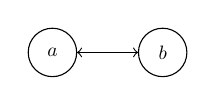
\begin{tikzpicture}[node distance=2cm]
\node[state, scale=0.7] (a) {$a$};
\node[state, scale=0.7] (b) [right of=a] {$b$};
\path[->] (a) edge [above] (b);
\path[->] (b) edge [below] (a);
\end{tikzpicture}
\vspace{1em}

$U$ satisfies Extensionality, but not Pairing or Foundation.
\vfill

\item $U=\{a,b,c\}$, $a \in c$, $b \in c$, $c \in c$

\vspace{1em}
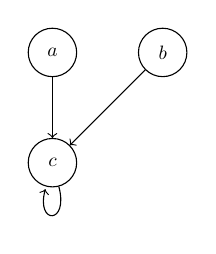
\begin{tikzpicture}[node distance=2cm]
\node[state, scale=0.7] (a) {$a$};
\node[state, scale=0.7] (b) [right of=a] {$b$};
\node[state, scale=0.7] (c) [below of=a] {$c$};
\path[->] (a) edge [above] (c);
\path[->] (b) edge [above] (c);
\path[->] (c) edge [loop below] (c);
\end{tikzpicture}

$U$ satisfies Pairing, but not Foundation or Extensionality.

\vfill

\item $U= \{a,b,c\}$, $a \in b$, $a \in c$, $b \in c$

\vspace{1em}
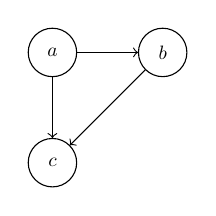
\begin{tikzpicture}[node distance=2cm]
\node[state, scale=0.7] (a) {$a$};
\node[state, scale=0.7] (b) [right of=a] {$b$};
\node[state, scale=0.7] (c) [below of=a] {$c$};
\path[->] (a) edge [above] (b);
\path[->] (a) edge [below] (c);
\path[->] (b) edge [above] (c);
\end{tikzpicture}

$U$ satisfies Extensionality and Foundation, but not Pairing.
\vfill
\end{enumerate}

\newpage


\item Let $R$, $S$, and $T$ be arbitrary relations (not necessarily functions). Show that $R \circ (S \circ T) = (R \circ S) \circ T$.

\begin{proof}
\ \\
We will show that $R \circ (S \circ T) = (R \circ S) \circ T$ by showing that each side is a subset of the other.
Let $x$ and $z$ be arbitrary elements of $dom(R \circ (S \circ T))$.
Then there exists a $y$ such that $\langle x,y \rangle \in R$ and $\langle y,z \rangle \in S \circ T$.
This means that there exists a $w$ such that $\langle y,w \rangle \in S$ and $\langle w,z \rangle \in T$.
Therefore $\langle x,w \rangle \in R \circ S$ and $\langle w,z \rangle \in T$.
So $\langle x,z \rangle \in (R \circ S) \circ T$.
Therefore $dom(R \circ (S \circ T)) \subseteq (R \circ S) \circ T$.
Now let $x$ and $z$ be arbitrary elements of $dom((R \circ S) \circ T)$.
Then there exists a $w$ such that $\langle x,w \rangle \in R \circ S$ and $\langle w,z \rangle \in T$.
This means that there exists a $y$ such that $\langle x,y \rangle \in R$ and $\langle y,w \rangle \in S$.
Therefore $\langle y,z \rangle \in S \circ T$.
So $\langle x,z \rangle \in R \circ (S \circ T)$.
Therefore $(R \circ S) \circ T \subseteq R \circ (S \circ T)$.
Therefore $R \circ (S \circ T) = (R \circ S) \circ T$.
\end{proof}

\newpage

\item Recall that the successor of a set $x$ is defined as $S(x) = x \cup \{ x \}$. Prove that if $x$ and $y$ are ordinals with $S(x)=S(y)$, then $x=y$. 

\vspace{1em}
\begin{proof}
\ \\
Let $x$ and $y$ be ordinals such that $S(x) = S(y)$.
Then $S(x) = x \cup \set{x}$ and $S(y) = y \cup \set{y}$.
We have seen before that if $\alpha \in ON$ then $S(\alpha) \in ON$.
So $S(x)$ and $S(y)$ are ordinals.
Now let us assume $x \neq y$.
So either $x \in y$ or $y \in x$.
We know $x \in S(x)$ and therefore $x \in S(y)$.
If $x \in S(y)$ then $x \in y$ or $x = y$.
But $x \neq y$ so then $x \in y$ must be the case.
However by the same logic $y \in x$ must also be the case.
This is a contradiction as it implies $x = y$ so $x = y$ must be the case.
\end{proof}
\newpage


\item Recall the lexicographic product from the previous homework. Show that if $(X, <)$ and $(Y, \prec)$ are well-orders, then so is their lexicographic product.

\vspace{1em}
\begin{proof}
 \ \\
A relation $R$ well-orders a set $A$ if R totally orders $A$ strictly and $R$ is well-founded on $A$.
We have shown that the lexicographic product is a strict total order, so we need to show that it is well-founded.
A relation is well-founded if every non-empty subset of the domain has an $R$-minimal element.
Since $X$ and $Y$ are well-ordered, every non-empty subset of $X$ and $Y$ has an $<$-minimal and $\prec$-minimal elements respectively.
The lexicographic product is defined as $\forall x_i \in X y_i \in Y (x_1,y_1) <_{\text{lex}} (x_2,y_2) \ \Leftrightarrow\ (x_1<x_2) \vee (x_1=x_2 \wedge y_1 \prec y_2)$.
We can see that if $x_{min}$ is the $<$-minimal element of $X$ and $y_{min}$ is the $\prec$-minimal element of $Y$, then $(x_{min},y_{min})$ is the $<_{\text{lex}}$-minimal element of $X \times Y$.
As $\forall (x_i,y_i)$ in $X \times Y$ we have $(x_{min},y_{min}) <_{\text{lex}} (x_i,y_i)$ or $(x_{min},y_{min}) = (x_i,y_i)$.
That is $\neg \exists (x,y) ((x,y) \in X \times Y \wedge (x,y)<_{lex} (x_{min},y_{min}))$.
Because otherwise either $x < x_{min}$ or $x = x_{min} \wedge y \prec y_{min}$.
And neither of these are possible so $(x_{min},y_{min})$ is the $<_{\text{lex}}$-minimal element of $X \times Y$.
\end{proof}
\end{enumerate}



\end{document}
